%\subsection{Pedagogical development}

%The first section describes "How do you get people to learn things?", cognitive psychology. Often school is studied, where learning is about being taught a subject, and then to pass a test. E-learning tools are often designed to do similar things to what schools does.

%The second section describes "How do you get people to behave differently?", social psychology. One area of research is about building habits. This is highly relevant in e-learning, where behavior change may be necessary to build the habit of using an app or a digital tool repeatedly.

%\include{theory/learning/pedagogical-development/cognitive_psychology}

%\subsubsubsection{Learning}

  \subsubsection{Learning the Right Things: Mapping educational objectives with Bloom's Revised Taxonomy}

  What to teach should be determined by the learning objectives of the activity.

  Depending on the objective, it fits differently into the Knowledge dimension and Cognitive Process dimension of Bloom's Revised Taxonomy. \cite{bloom}

  The taxonomy provides a framework for determining and clarifying learning objectives. See figure \ref{fig:revised-bloom} from \cite{heer}. Each colored block is an example of a learning objective matching with the two dimensions. The image also explains the different concepts.

  \begin{figure}[h]
    \centering
    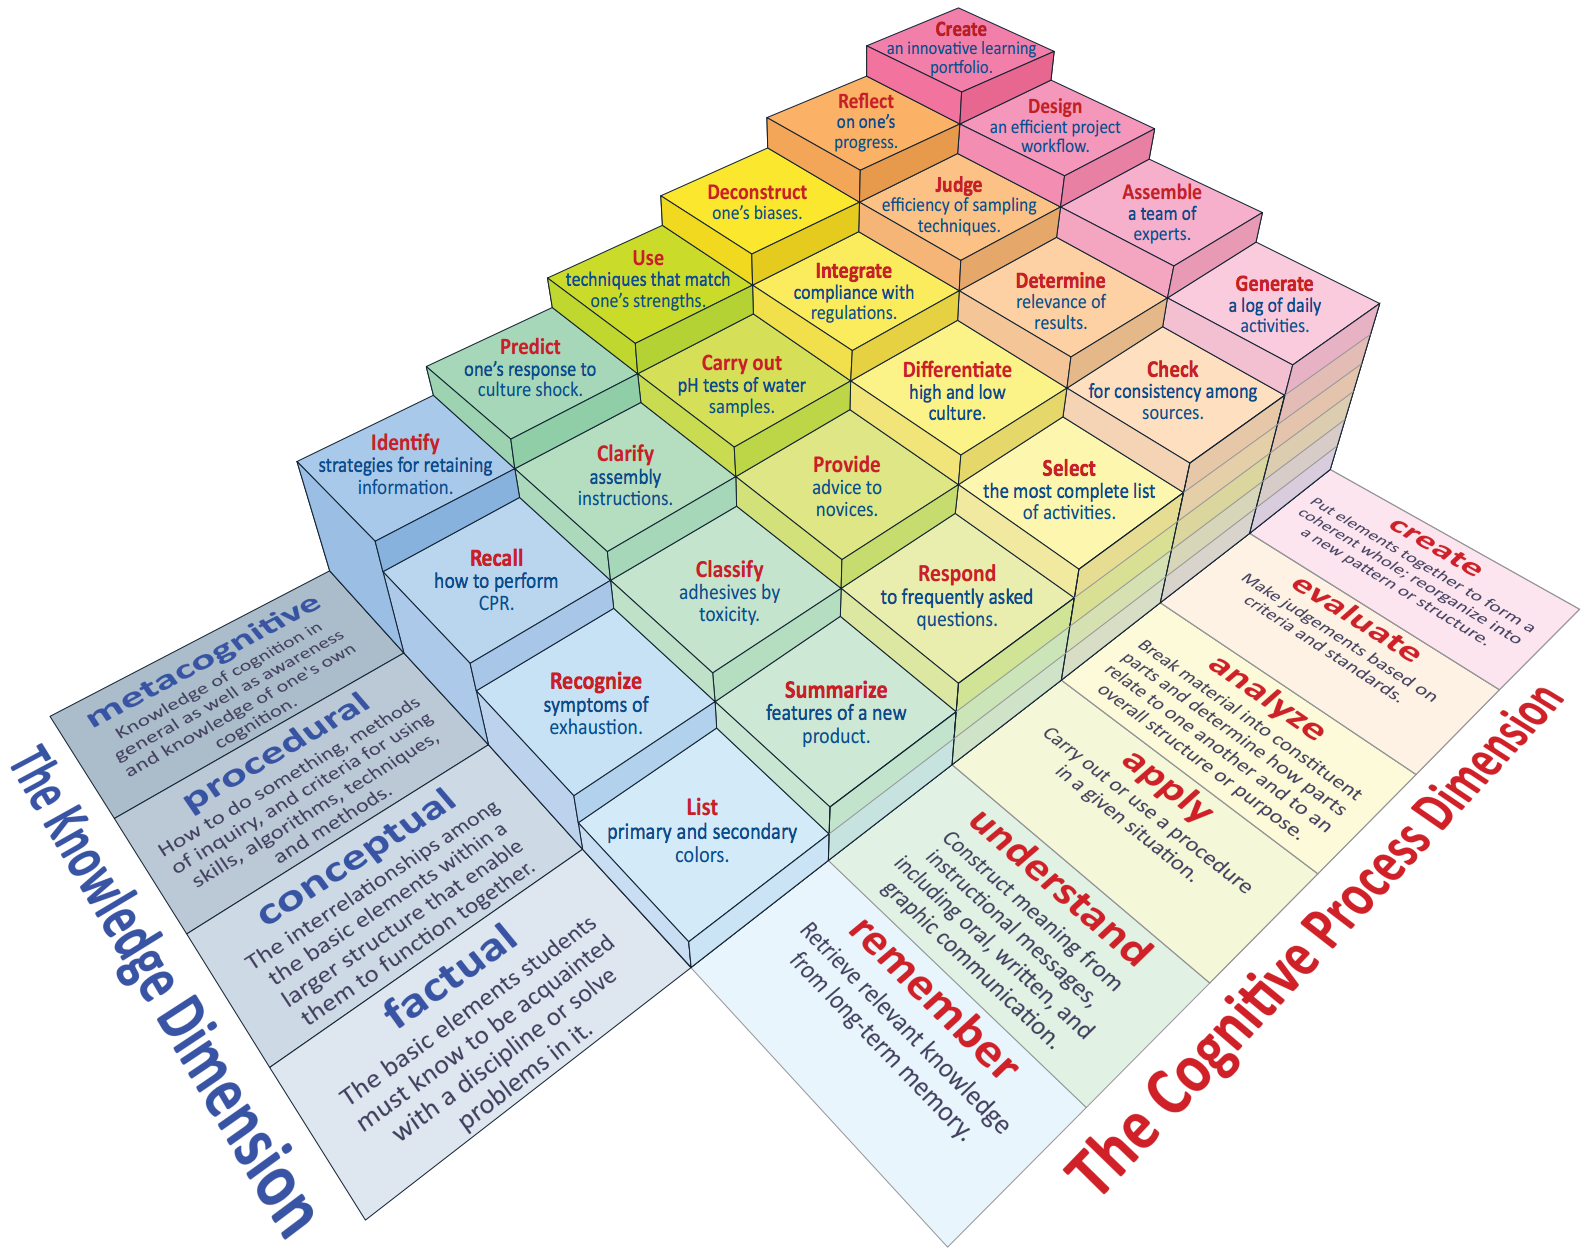
\includegraphics[width=1.0\textwidth]{RevisedBloom.png}
    \caption{Bloom's revised taxonomy visualised with examples of different learning objectives.}
    \label{fig:revised-bloom}
\end{figure}

  Learning activities often involve both lower order and higher order thinking skills as well as a mix of concrete and abstract knowledge.

  The taxonomy can provide usable insight into how to design, by the combination between lower or higher cognitive complexity, and concrete (factual or conceptual) or abstract knowledge (procedural or metacognitive). \cite{cheong}

  \subsubsection{Building skills: by Spaced practice, Deliberate practice and Perceptual exposure}

  Spaced practice deals with spreading out learning, with the purpose of not forgetting. E.g. Gates \cite{Gates} concludes that spaced learning versus massed learning did have a memory benefit in their study.

  Designing for this, could mean making the user apparent on the person's meta-cognitive ability (personal insight into what you'll remember), and meta-memory (when you need to repeat information in order not to forget).

  Moreover, dividing learning into 45-90-minute chunks, getting to 95\% reliable within one to three sessions, has been proven highly effective. This is called deliberate practice. Gates \cite{Gates} agrees, finding no evidence of consistent correlation between total duration and effects on learning outcomes in their study. Sierra says, if you can’t get the user to 95\% reliability within this time, stop trying; you need to redesign the sub-skill. \cite{sierra}

  Sierra presents a number of strategies, most notably research within deliberate practice \cite{yengin} \cite{sierra}. Deliberate practice has been proven to be an effective way to build skills. It has also been tested before for mobile learning environments. \cite{yengin}

  Sierra \cite{sierra} suggests skills to be divided into three buckets: can't do (but need to do), can do with effort, and mastered (reliable/automatic). The goal then is to move skills from can't do into mastered, in the best way possible. See figure \ref{fig:sierra-practice} from Sierra \cite{sierra}.

  \begin{figure}[h]
    \centering
    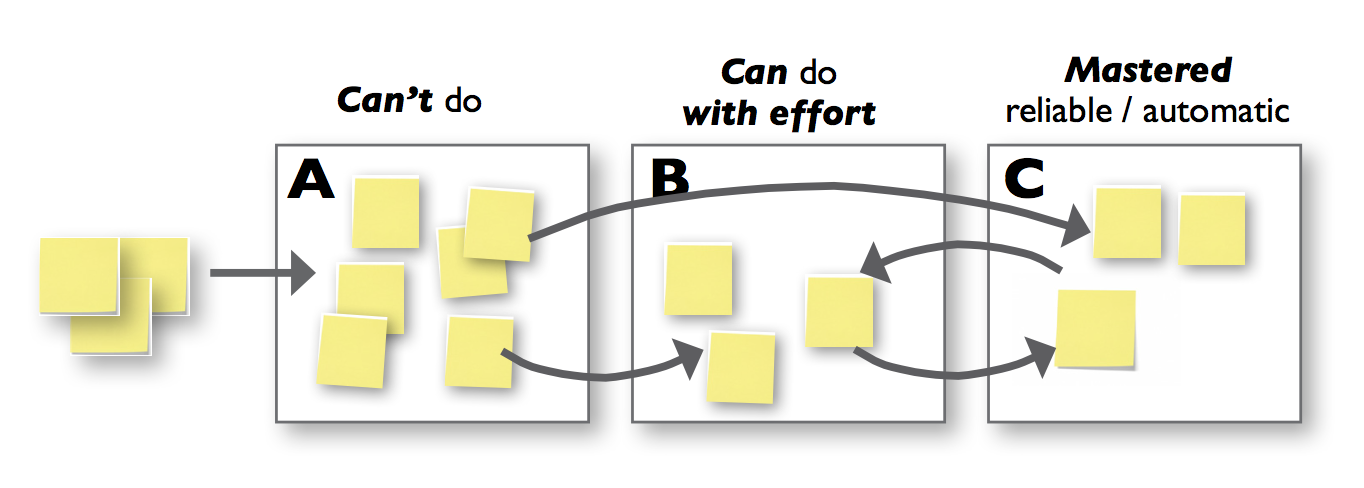
\includegraphics[width=0.8\textwidth]{SierraPractice.png}
    \caption{Moving skills from A (Can't do) to B (Can do with effort) into C (Mastered) can move different ways, depending on how effective the learning is. Deliberate practices focuses on A-B-C, while perceptual expose enables A to C. Reflection allows knowledge to go backwards, to get better at the skill than previously possible.}
    \label{fig:iterationprocess}
\end{figure}

  Desirable difficulties applies here, meaning that during deliberate practice, it may feel as if learning gets harder and harder, but in the long term the user is actually learning more. As a result, less people does true deliberate practice, but they do not get the same reward in return. This needs to be designed for, e.g. using social psychology.

  A way to build skills quickly, is to utilize that the brain is brilliant at pattern-matching, by the method "perceptual exposure". \cite{sierra}

  Sierra shows how researchers have repeatedly, by well designed tests, been able to quickly build expertise by trial-and-error feedback. A novice would hazard a guess and an expert would say yes or no. Eventually the novices became, like their mentors, masters of the expertise that could otherwise would have been intangible for long.

  Whenever a skill relies on intuition, we could try exposing the user a well-designed trail and error test. This is done by exposing users to very high-quality samples during a very limited time. Perceptual knowledge includes teaching what we think of as expert intuition (like being a good entrepreneurship coach).

  \subsubsection{Learning from Assessment}

  Knowing what learners know, and don't know, is crucial to effective learning, Luckin \cite{luckin} says.

  Assessment can partly help to design for flow, matching challenge and ability \cite{bruhlmann}, which is effective for intrinsic motivation (see next chapter).

  Moreover, it also has cognitive benefits. It can help to offer appropiate feedback, increase learners' awareness of their learning needs, and give accurate assessment and analysis, and allows learning to be tailored.

  By recognizing differences of students, in their ability to understand what they know and how they can progress, it is possible to ensure that everyone achieves their full potential.

  Effective assessment by a teacher or agent includes individual feedback (task-oriented and informal) and appropiate feed-forward advice.

  \subsubsection{Learning by Thinking: Reflection \& Retrieval Practice}

  When reflecting, the student develops neccessary skills and self-awareness to refine their own learning activities. This surely applies to the teacher as well, Luckin says. \cite{luckin}

  Stefano \cite{stefano} suggests that that reflection has been an overlooked area of research for a long time.

  They found that individuals who are given time to reflect on a task, outperforms students who are given the same amount of time to practice with the same task.

  His results suggests that reflection as an activity that can be more effective than additional learning.

  Similar to deliberate practice, it is a desirable difficulty. Individuals in the test themselves, had a tendancy to allocate time to practice on the task rather than reflecting on it.

  %\subsubsection{Retrieval practice}

  Bjork \cite{bjork} shows that retrieval from memory is more effective than people who repeat reading the same thing to remember.

  They also showed, that the more effective students, retrieves from memory.

  E.g. "What was in that article?", instead of immediately reading the article, is an example of memory retrieval that is extremely effective for learning, their research shows.

  One design method to encourage this, would be flip cards, where the question is on one side, the answer is on the other, versus giving the person a multiple-choice question.

%\subsubsection{Not forgetting}

%UCLA Bjork's Learning and Forgetting Lab researches how people forget, and how to design so that people do not forget.

%\include{theory/learning/pedagogical-development/social_psychology}
